%%%%%%% Euclidean Geometry Course Notes %%%%%%%%%%%%%%%%
%%%%%%% Supplemental Sequence on Trigonometry %%%%%%%%%%%%%%%%

\documentclass{amsart}
\usepackage[margin=1in]{geometry}
\usepackage{arcs}
\usepackage{graphicx}
\usepackage{multicol}
\usepackage[final]{pdfpages}


\theoremstyle{definition}
%\newtheorem{letterconj}{Conjecture}
%\newtheorem{letterchallenge}[letterconj]{Challenge}
%\newtheorem{letterquestion}[letterconj]{Question}
%\newtheorem{letterprob}[letterconj]{Problem}


\swapnumbers
\newtheorem{problem}{Problem}[section]
\newtheorem{conjecture}[problem]{Conjecture}
\newtheorem*{definition}{Definition}
\newtheorem*{theorem}{Theorem}
\newtheorem{question}[problem]{Question}
\newtheorem{challenge}[problem]{Challenge}
\newtheorem*{postulate}{Postulate}

\begin{document}

\title{Euclidean Geometry Supplement}
\author[Euclidean Geometry]{Trigonometry from the Ground Up}

\maketitle

\setcounter{section}{0}
\renewcommand{\thesection}{\Alph{section}}
\section{The Arithmetic of Segments: Addition and Comparison}

Euclid uses his Common Notions to cover a lot of ground. At least one place where we can do a bit better if we put in the effort is in discussing how we handle addition and subtraction of segments.

\begin{definition} Let $AB$ and $CD$ be two segments. We say that $AB$ is \emph{less than} $CD$ when there exists a point $M$ lying between $C$ and $D$ such that $AB$ is congruent to $CM$. Sometimes we will say that $CD$ \emph{is greater than} $AB$, which means the same thing.
\end{definition}

\begin{conjecture} If $AB$, $CD$ and $EF$ are segments such that $AB$ is less than $CD$ and $CD$ is less than $EF$ then $AB$ is less than $EF$.
\end{conjecture}

\begin{definition}
Let $AB$ and $CD$ be segments. We define a new segment $AE$ called the \emph{sum of $AB$ and $CD$} as follows: Extend the segment $AB$ to a ray from $A$ through $B$, and choose a point $E$ on the ray so that 
\begin{enumerate}
\item $B$ lies between $A$ and $E$, and 
\item $BE$ is congruent to $CD$.\end{enumerate} 
We shall write $AB+CD$ for the sum of the two segments.
\end{definition}

\begin{conjecture} If $AB$ is a segment, then $AB+AB$ may not be equal to $BA+BA$ but these two new segments are congruent. [Related question: How does $AB+BA$ fit into this picture?]
\end{conjecture}



\begin{definition}\label{defn:segment-class} 
Let $AB$ be a segment. By the \emph{class} of $AB$, we mean the set of all segments $CD$ such that $CD$ is congruent to $AB$.
\end{definition}

\begin{conjecture} Let $a$ and $b$ be segment classes. Then exactly one of the following holds:
\begin{itemize}
\item[(i)] $a\cap b = \emptyset$, or
\item[(ii)] $a = b$.
\end{itemize}
\end{conjecture}


\begin{definition}\label{defn:sum-segment-classes} 
Let $a$ and $b$ be segment classes. We define the sum $a+b$ to be the class of the segment $AB+CD$, where $AB$ is an element of the class of $a$ and $CD$ is an element of the class $b$.
\end{definition}

\begin{problem} 
The notion of sum of classes does not depend on the particular choices of segments $AB$ and $CD$.
\end{problem}


\begin{problem}
Let $a$ and $b$ be segment classes. Then $a+b = b+a$.
\end{problem}

\begin{problem}
Let $a, b, c$ be segment classes. Then $(a+b)+c = a + (b+c)$.
\end{problem}

\begin{problem} 
Let $a, b$ be segment classes. Then one and only one of the following holds:
\begin{itemize}
\item[(i)] $a=b$;
\item[(ii)] There is a class $c$ such that $a+c=b$;
\item[(iii)] There is a class $c$ such that $a= b+c$.
\end{itemize}
\end{problem}

\begin{problem} 
Show that the notion of ``less than'' extends unambiguously to segment classes.
\end{problem}

\begin{problem}
Let $a, b, c$ be segment classes such that $a$ is less than $b$. Then $a+c$ is less than $b+c$.
\end{problem}

%%%%%%%%%%%%%%%%%%%%%%%%%%%%%%%%%%%%

\vfill
\pagebreak


\setcounter{section}{1}
\renewcommand{\thesection}{\Alph{section}}
\section{Arithmetic of Segments: Multiplication}



\begin{center}
\textbf{Once and for all, choose a segment $XY$ and declare the class of this segment to be the unit class $1$.}
\end{center}

\begin{definition}
Let $a,b$ be two segment classes. We define their \emph{product} $a\cdot b$ as follows:

Let $AB\in 1$ and construct a segment $BC \in a$ which is perpendicular to $AB$. This forms a right triangle $ABC$. Next construct a right triangle $DEF$ with angle $E$ a right angle, angle $D$ congruent to angle $A$ and $DE \in b$. Then $a\cdot b$ is the class of $EF$.
\end{definition}

\begin{center}
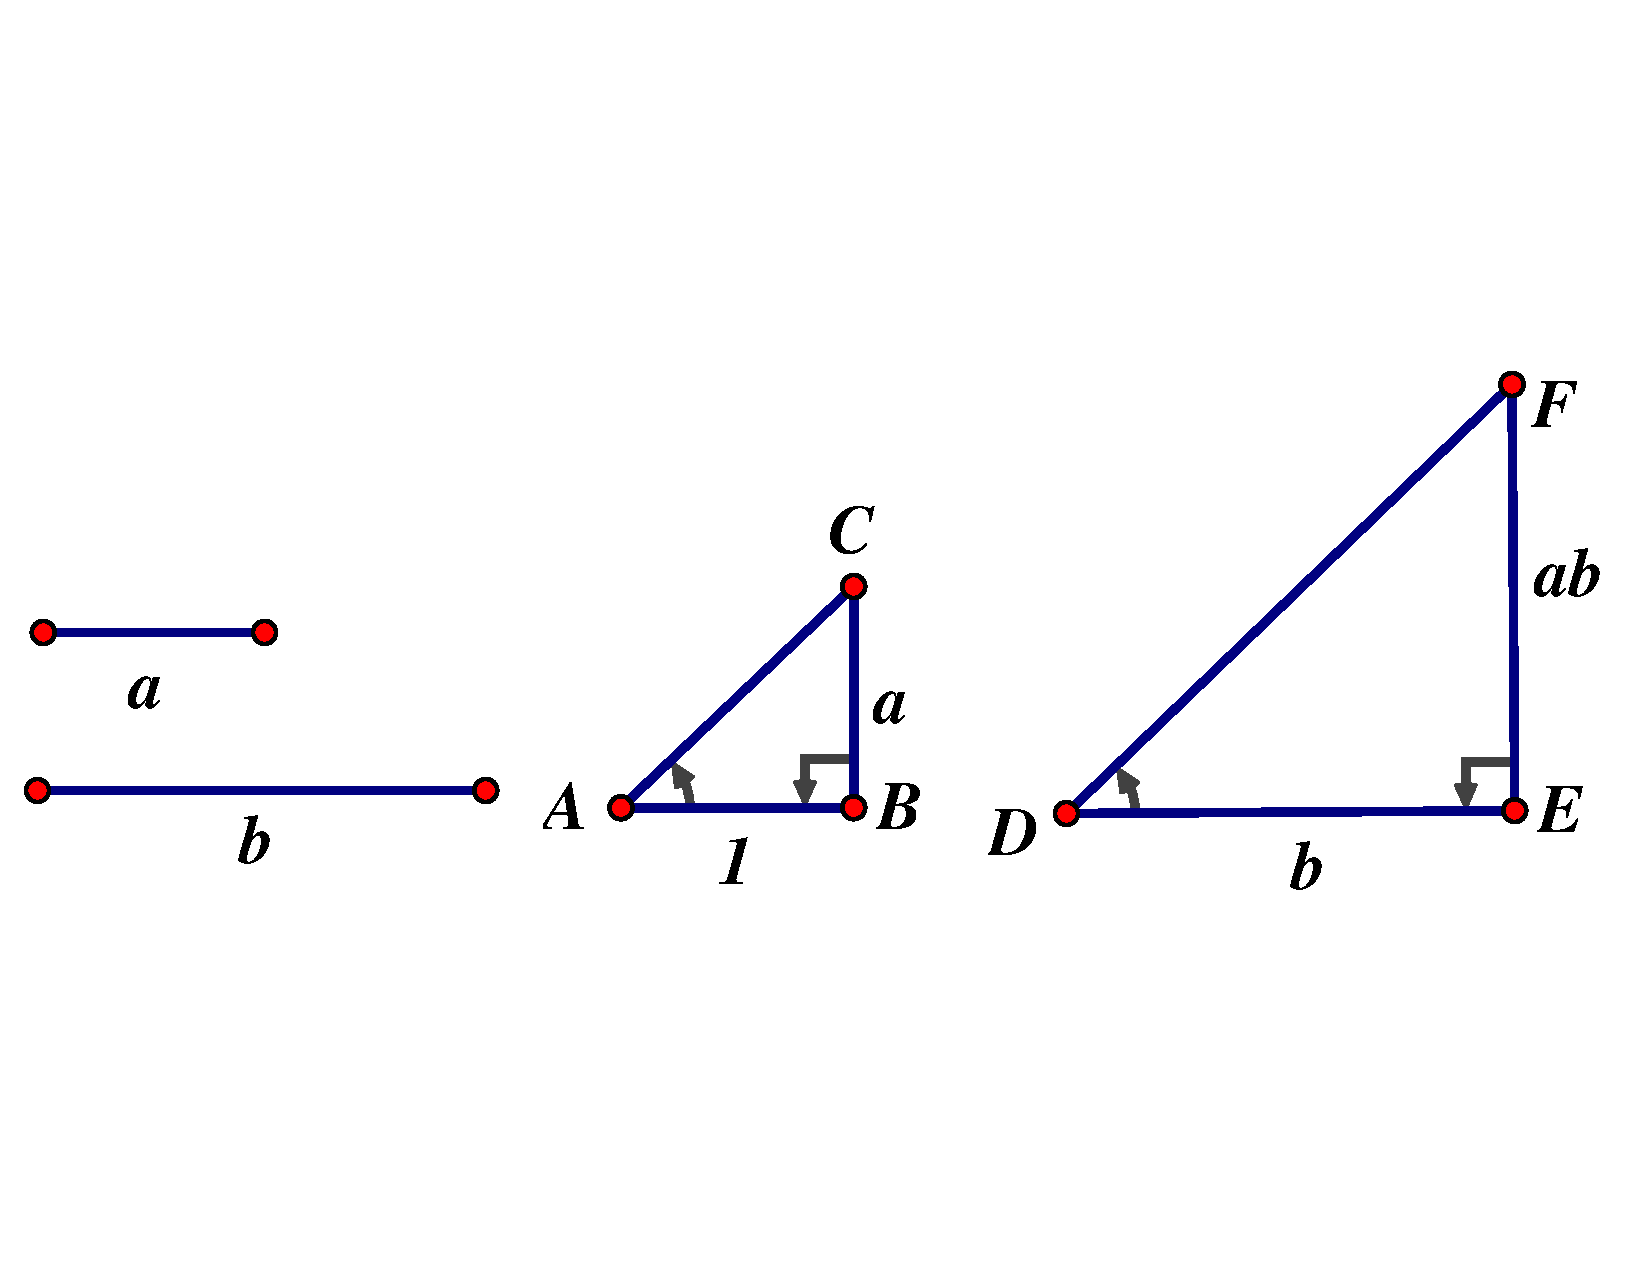
\includegraphics[scale=.4]{product.pdf}
\end{center}

\begin{problem}
Show that this definition makes sense because the constructions can be carried out, and also the end result does not depend on the choices made.
\end{problem}

We wish to have several ``algebraic properties'' for this operation. That is the content of the next five problems.

\begin{conjecture} \label{problem:segment-class-structure}
For any segment class $a$, it is true that $a\cdot 1 = a$.
\end{conjecture}

\begin{conjecture} 
For any segment classes $a, b$, it is true that $a\cdot b = b\cdot a$.
\end{conjecture}

\begin{conjecture} 
For segment classes $a, b, c$, it is true that $a\cdot (b\cdot c) = (a\cdot b) \cdot c$.
\end{conjecture}

\begin{conjecture} 
For any segment class $a$, there is a unique segment class $b$ so that $a\cdot b = 1$.
\end{conjecture}

\begin{definition} The class constructed in the last Conjecture is called the \emph{inverse} of $a$ and denoted $a^{-1}$. In what follows, we will sometimes have the occasion to form a product like $d \cdot a^{-1}$ and in this case we may write $d/ a$ or $\dfrac{d}{a}$ instead.
\end{definition}

\begin{conjecture} 
For segment classes $a, b, c$, it is true that $a\cdot (b + c) = a\cdot b + a\cdot c$.
\end{conjecture}

Now we can define our trigonometric functions.

\begin{definition}\label{defn:trig-fns}
Let $\alpha$ be a given angle. We define a pair of segment classes called the \emph{sine of $\alpha$} and the \emph{cosine of $\alpha$} as follows: 

Construct a right triangle $ABC$ with hypotenuse $AC$ in the unit segment class $1$, and angle $CAB$ congruent to $\alpha$. Then the \emph{sine} of $\alpha$ is the class of $BC$ and is denoted $\sin \alpha$, and the \emph{cosine} of $\alpha$ is the class of $AB$ and is denoted $\cos \alpha$.
\end{definition}


\begin{problem}\label{prob:defn-trig}
Suppose that angle $\alpha$ is less than a right angle. Show that the construction required in the last definition is both possible and unambiguous. (So $\sin\alpha$ and $\cos\alpha$ make sense.)
\end{problem}


\vfill
\pagebreak

\section{Similar Triangles}

Our work on multiplication hinges on knowing about triangles which have corresponding angles the same, but sides which differ. Let us explore this idea.

\begin{definition} We say that two triangles $ABC$ and $DEF$ are \emph{similar} when 
\begin{itemize}
\item $\angle A \cong \angle D$, $\angle B \cong \angle E$ and $\angle C \cong \angle F$, and 
\item there exists a segment class $\lambda$ such that 
\[
AB = \lambda \cdot DE, \quad BC = \lambda \cdot EF, \mbox{ and } CA = \lambda\cdot FD.
\]
\end{itemize}
When this definition is satisfied, we may denote the relationship that $ABC$ is similar to $DEF$ by the symbol $ABC \sim DEF$.
\end{definition}

Note that we are being sloppy about multiplying segments and segment classes. At this point, there should be no confusion that always we really multiply segment classes, but sometimes we may denote a class by one of its representatives.

Like the definition of triangle congruence, this definition has a lot in it to check. We want to develop some theorems that give sufficient conditions for similarity and have shorter lists of things to verify. Our main goal is this:

\begin{theorem}[The Similarity Theorem] Two triangles are similar if and only if two of the three pairs of corresponding angles are congruent.
\end{theorem}

To prove this result, we will work through a sequence of partial results.

\begin{problem} Prove the Similarity Theorem under the additional hypotheses that 
\begin{itemize}
\item all three pairs of corresponding angles are congruent, and
\item both triangles are right triangles.
\end{itemize}
\end{problem}

\begin{problem} Prove the Similarity Theorem under the additional hypothesis that all three pairs of corresponding angles are congruent.
\end{problem}

\emph{Hint: How can we decompose an arbitrary triangle into some right triangles? Think about the proof of the theorem on existence of the incenter.}

\begin{problem} Prove the Similarity Theorem without any additional hypothesis.
\end{problem}



\begin{conjecture}[SAS Similarity] Suppose that $ABC$ and $DEF$ are triangles such that $\angle A$ is congruent to $\angle D$ and there exists a segment class $\lambda$ such that $AB = \lambda\cdot DE$ and $AC= \lambda\cdot DF$. Then $ABC$ is similar to $DEF$.
\end{conjecture}


Next, we want a generalization of the Midline Theorem that clarifies the relationship between``proportionality'' of segments and parallelism.

\begin{conjecture} Let $ABC$ be a triangle. Extend sides $AB$ and $AC$ to rays emanating from $A$. Let $\ell$ be a line which cuts across these two rays at points $D$ and $E$, respectively. Then $\ell$ is parallel to $BC$ if and only if 
\[
\dfrac{AB}{AD} = \dfrac{AC}{AE}.
\]
\end{conjecture}


\begin{problem} We have a variety of triangle congruence theorems. Which ones can be adjusted to give similarity theorems? State and prove some theorems.
\end{problem}


%%%%%%%%%%%%%%%%%%%%%%%%%%%%%%%%%%%%%%%%%%%%%%%%%%%%%55


\vfill
\pagebreak

\section{The Anatomy of an Altitude}
Let $ABC$ be a triangle. The \emph{altitude} of the triangle through $C$ is the line segment from $C$ to the line through $A$ and $B$ which is perpendicular to that line. I want to introduce a bunch of terminology and notation quickly, so I'll use a diagram.

\begin{center}
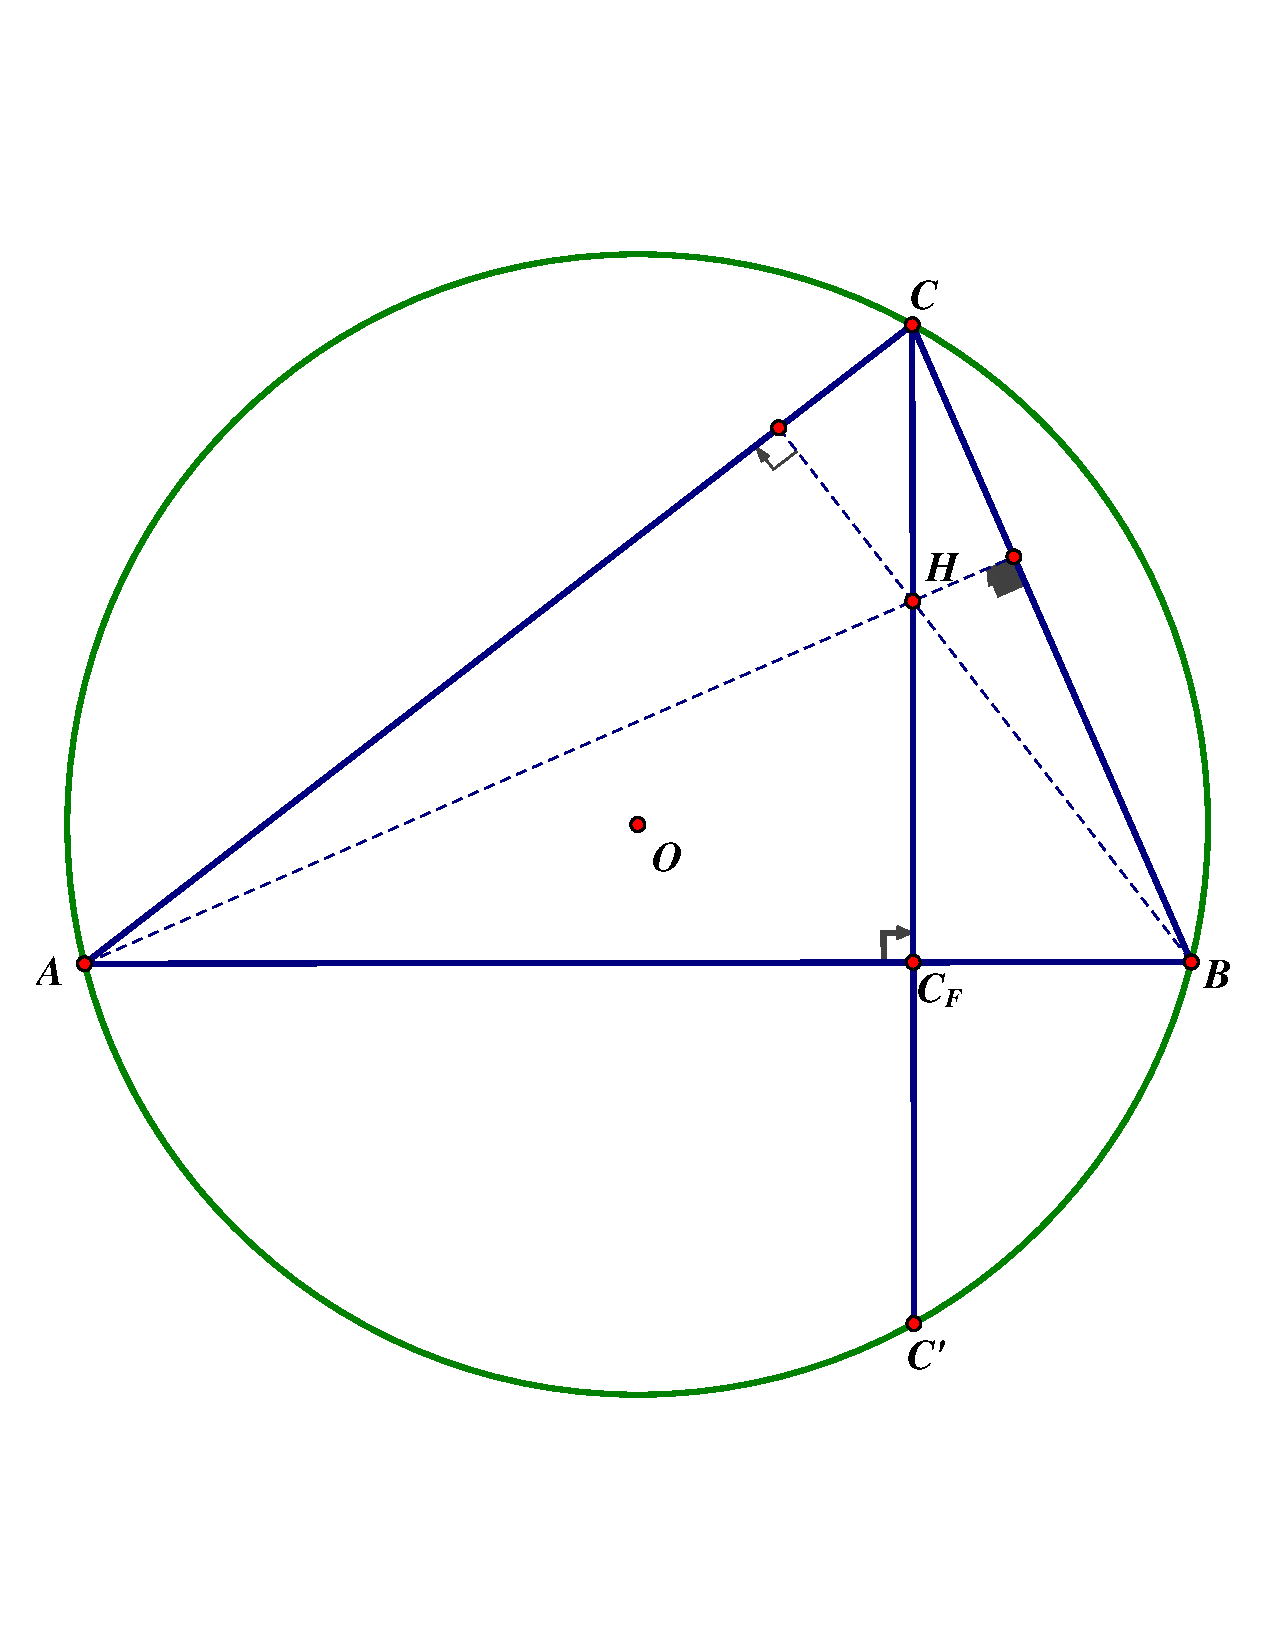
\includegraphics[scale=.4]{Anatomy-of-Altitude.pdf}
\end{center}

Let $O$ be the circumcenter of the triangle $ABC$. Then
\begin{multicols}{3}
\begin{itemize}
\item[] $CC_F = $ altitude
\item[] $C_F = $ foot
\end{itemize}
\begin{itemize}
\item[] $C_FC' = $ root
\item[] $H = $ orthocenter
\end{itemize}
\begin{itemize}
\item[] $CH = $ ear
\item[] $HC_F = $ stem
\end{itemize}
\end{multicols}

\begin{problem} \label{prob:orthocenter}
Show that the three altitudes of a triangle are concurrent. (The point of concurrence is called the \emph{orthocenter}.)
\end{problem}

\begin{conjecture} \label{prob:sine-in-circle}
Let triangle $ABC$ be inscribed in a circle whose diameter is a unit segment. Suppose that all three internal angles of $ABC$ are less than a right angle. Show that $AB \in \sin(\angle ACB)$.
\end{conjecture}

\begin{conjecture} \label{prob:cosine-in-circle}
Let triangle $ABC$ be inscribed in a circle whose diameter is a unit segment. Suppose that all three internal angles of $ABC$ are less than a right angle. Show that $CH \in \cos(\angle ACB)$.
\end{conjecture}



\begin{problem} Suppose that $\alpha$ is an angle which is congruent to or greater than a right angle. Find a geometric way (using our diagram) to interpret $\sin\alpha$ and $\cos\alpha$. Can these segment classes be related to the sine or cosine of some angles that are less than a right angle?
\end{problem}

\begin{conjecture}
A circle through any three of the four points $A, B, C, H$ will have the same diameter as any of the other possible choices.
\end{conjecture}

\begin{conjecture}
The stem and root of an altitude are congruent.
\end{conjecture}

\begin{problem}[More Trigonometry]\label{prob:trig-fns-cont}
Use our basic picture of an acute triangle inscribed in a circle with unit diameter to give geometric descriptions to the other basic trigonometric functions: (a) $\tan \alpha$, (b) $\sec \alpha$, (c) $\cot \alpha$, and (d) $\csc \alpha$.
\end{problem}

\vfill
\pagebreak

\section{Even More Trigonometry}


\begin{conjecture}[The Law of Sines]
If $ABC$ is inscribed in a circle of diameter $d$, then $AB \in d\cdot \sin(\angle C)$, $BC \in d\cdot \sin(\angle A)$, $AC \in d\cdot \sin(\angle B)$.
\end{conjecture}

In modern terms, the last result is stated more like this: If a triangle has angles $\alpha, \beta$ and $\gamma$ opposite sides $a, b$ and $c$, respectively, and also has circumscribed circle of radius $R$, then
\[
\dfrac{a}{\sin(\alpha)} = \dfrac{b}{\sin(\beta)} = \dfrac{c}{\sin(\gamma)} = 2R
\]



\begin{conjecture}
Continuing the last conjecture, and recalling that $H$ is the orthocenter, we have the relations $AH \in d\cdot \cos(\angle A)$, $BH \in d\cdot \cos(\angle B)$, and $CH \in d\cdot \cos(\angle C)$.
\end{conjecture}



\begin{conjecture}
Let $ABCD$ be a cyclic quadrilateral. Then there exists a point $K$ on the segment $AC$ so that $\triangle ABK$ is similar to $\triangle DBC$.
\end{conjecture}



\begin{problem}[Ptolemy's Theorem]\label{prob:ptolemy-theorem}
Let $ABCD$ be a cyclic quadrilateral, and suppose it is simple. Then
\[  
AC\cdot BD = AB\cdot CD + AD\cdot BC
\]
\end{problem}

\begin{problem}
Show if $D$ does not lie on the circumcircle of triangle $ABC$, then the left-hand side is always strictly less than the right-hand side.
\end{problem}

This result is due to Ptolemy, an astronomer-mathematician from Alexandria, and it is one of my favorite theorems. One can view it as a way of characterizing the points lying on a circle. The three points $A, B, C$ define a circle, the circumcircle of triangle $ABC$. Then the theorem tells us a way to decide if a fourth point $D$ lies on the circle or not. If you know something about ancient astronomy, you will recognize why Ptolemy thought this was important thing. \\


\begin{problem}
Use Ptolemy's theorem to show that for a convex regular pentagon, if $a$ is the segment class of the side and $b$ is the segment class of a diagonal, then $\varphi = b\cdot a^{-1}$ is the golden ratio. That is, $\varphi$ is the positive root of the equation $\varphi^2 = 1+ \varphi$.
\end{problem}


One can base a pretty thorough understanding of trigonometry on Ptolemy's theorem. The last sequence of problems consists of trigonometric identities.

\begin{problem} $(\sin\alpha)^2 + (\cos\alpha)^2 = 1$
\end{problem}

\begin{problem} Use Ptolemy's theorem to prove the Law of Cosines: Let $ABC$ be a triangle. If $a$, $b$ and $c$ are the segment classes of the sides opposite vertices $A, B$ and $C$, respectively, then
\[
c^2 + 2a b \cos(\angle ACB)= a^2 + b^2
\]
\end{problem}

\begin{problem} Explain how the law of cosines is related to Euclid's Propositions II.12 and II.13.
\end{problem}

\begin{problem}
$\sin(\alpha + \beta) = \cos\alpha \sin\beta + \cos\beta\sin\alpha$
\end{problem}


\begin{problem}
$\cos(\alpha + \beta) = \cos\alpha\cos\beta - \sin\alpha\sin\beta$
\end{problem}


\begin{problem}
$\cos(\alpha - \beta) = \sin\alpha\sin\beta + \cos\alpha\cos\beta$
\end{problem}


\begin{problem}
$\tan \alpha + \tan\beta = \dfrac{\sin(\alpha + \beta)}{\cos\alpha\cos\beta}$
\end{problem}


\vfill
\pagebreak

%%%%%%%%%%%%%%%%%%%%%%%%%%%%%%%%%%%%%%

%idea for a new set of problems: constructing a tangent to a different conic--old school! with similarity and definition of a conic using focus-directrix quadratic expressions\dots
%
%\vfill
%\pagebreak

\end{document}